\documentclass[]{article}
\usepackage{lmodern}
\usepackage{amssymb,amsmath}
\usepackage{ifxetex,ifluatex}
\usepackage{fixltx2e} % provides \textsubscript
\ifnum 0\ifxetex 1\fi\ifluatex 1\fi=0 % if pdftex
  \usepackage[T1]{fontenc}
  \usepackage[utf8]{inputenc}
\else % if luatex or xelatex
  \ifxetex
    \usepackage{mathspec}
    \usepackage{xltxtra,xunicode}
  \else
    \usepackage{fontspec}
  \fi
  \defaultfontfeatures{Mapping=tex-text,Scale=MatchLowercase}
  \newcommand{\euro}{€}
\fi
% use upquote if available, for straight quotes in verbatim environments
\IfFileExists{upquote.sty}{\usepackage{upquote}}{}
% use microtype if available
\IfFileExists{microtype.sty}{%
\usepackage{microtype}
\UseMicrotypeSet[protrusion]{basicmath} % disable protrusion for tt fonts
}{}
\usepackage[margin=1in]{geometry}
\usepackage{longtable,booktabs}
\usepackage{graphicx}
\makeatletter
\def\maxwidth{\ifdim\Gin@nat@width>\linewidth\linewidth\else\Gin@nat@width\fi}
\def\maxheight{\ifdim\Gin@nat@height>\textheight\textheight\else\Gin@nat@height\fi}
\makeatother
% Scale images if necessary, so that they will not overflow the page
% margins by default, and it is still possible to overwrite the defaults
% using explicit options in \includegraphics[width, height, ...]{}
\setkeys{Gin}{width=\maxwidth,height=\maxheight,keepaspectratio}
\ifxetex
  \usepackage[setpagesize=false, % page size defined by xetex
              unicode=false, % unicode breaks when used with xetex
              xetex]{hyperref}
\else
  \usepackage[unicode=true]{hyperref}
\fi
\hypersetup{breaklinks=true,
            bookmarks=true,
            pdfauthor={},
            pdftitle={Methylation modules associate with incident cardiovascular disease and cumulative risk factor exposure},
            colorlinks=true,
            citecolor=blue,
            urlcolor=blue,
            linkcolor=magenta,
            pdfborder={0 0 0}}
\urlstyle{same}  % don't use monospace font for urls
\setlength{\parindent}{0pt}
\setlength{\parskip}{6pt plus 2pt minus 1pt}
\setlength{\emergencystretch}{3em}  % prevent overfull lines
\setcounter{secnumdepth}{5}

%%% Use protect on footnotes to avoid problems with footnotes in titles
\let\rmarkdownfootnote\footnote%
\def\footnote{\protect\rmarkdownfootnote}

%%% Change title format to be more compact
\usepackage{titling}

% Create subtitle command for use in maketitle
\newcommand{\subtitle}[1]{
  \posttitle{
    \begin{center}\large#1\end{center}
    }
}

\setlength{\droptitle}{-2em}

  \title{Methylation modules associate with incident cardiovascular disease and
cumulative risk factor exposure}
    \pretitle{\vspace{\droptitle}\centering\huge}
  \posttitle{\par}
    \author{}
    \preauthor{}\postauthor{}
    \date{}
    \predate{}\postdate{}
  
\usepackage{booktabs}
\usepackage{longtable}
\usepackage{array}
\usepackage{multirow}
\usepackage[table]{xcolor}
\usepackage{wrapfig}
\usepackage{float}
\usepackage{colortbl}
\usepackage{pdflscape}
\usepackage{tabu}
\usepackage{threeparttable}
\usepackage{threeparttablex}
\usepackage[normalem]{ulem}
\usepackage{makecell}

\usepackage{amsthm}
\newtheorem{theorem}{Theorem}[section]
\newtheorem{lemma}{Lemma}[section]
\theoremstyle{definition}
\newtheorem{definition}{Definition}[section]
\newtheorem{corollary}{Corollary}[section]
\newtheorem{proposition}{Proposition}[section]
\theoremstyle{definition}
\newtheorem{example}{Example}[section]
\theoremstyle{definition}
\newtheorem{exercise}{Exercise}[section]
\theoremstyle{remark}
\newtheorem*{remark}{Remark}
\newtheorem*{solution}{Solution}
\begin{document}

\maketitle


\section{Introduction}\label{introduction}

Genetic approaches to cardiovascular disease (CVD) research have led to
important breakthroughs in mechanistic understanding and therapeutic
strategies. However, the mechanisms for gene variant-disease
relationships are often difficult to determine, and their effects may
often be mediated by epigenetic regulation (M. J. Bonder et al. 2016).
DNA methylation is one such mechanism that can reflect both genetic
variation and environmental exposures and potentially drive their
effects on CVD outcomes (Ordov{á}s and Smith 2010).

A series of recent epigenome-wide association studies (EWAS) have
examined relationships between DNA methylation at
cytosine-phosphate-guanine (CpG) sites and various subtypes of CVD,
including prior myocardial infarction (Rask-Andersen et al. 2016), acute
coronary syndrome (J. Li et al. 2017), and atherosclerosis (Nakatochi et
al. 2017). These discoveries may reveal important mechanistic insights,
but are susceptible to reverse causation. Indeed, Mendelian
randomization approaches have suggested that reverse causation
(methylation being influenced by the phenotype of interest) is more
common (Dekkers et al. 2016; Wahl et al. 2017). One approach to this
problem is to examine epigenetic associations with cardiovascular risk
factors. Multiple investigations have explored these relationships
genome-wide (Pfeiffer et al. 2015; Irvin et al. 2014), and have even
uncovered prognostic CpG sites for incident coronary heart disease in
the process (Hedman et al. 2017; Aslibekyan et al. 2018). A few studies
looking directly at incident CVD as a binary variable have found
relationships with global DNA methylation (as approximated by LINE-1
methylation levels) and with a specific cluster of CpG sites in the
ZBTB12 gene (A. Baccarelli et al. 2010; Guarrera et al. 2015).

Most epigenetic investigations of CVD to-date have been performed in
blood, based on the importance of immune-related processes in its
pathogenesis (B{ä}ck and Hansson 2015) as well as its relative ease of
collection in comparison to other relevant tissues (e.g.~endothelium,
myocardium). In addition, several groups have shown a moderate ability
of blood-based methylomic signatures to reflect those in
disease-relevant tissues (Bacos et al. 2016; Y. T. Huang et al. 2016).

To address the problem of reverse causation while incorporating
time-to-event information, we set out to analyze relationships between
methylation and incident CVD using time-to-event models in a series of
two cohorts. Noting the previously-observed lack of replication in
CVD-related CpG sites (Fern{á}ndez-Sanl{é}s et al. 2017), we used
module- and region-based techniques to improve detection and the
robustness of findings. We sought context for two specific modules of
interest using gene- and chromatin-based annotations, and compared
module activations to past and current cardiovascular risk factor levels
to better understand their potential biological mechanisms.

\section{Results}\label{results}

\subsection{Weighted correlation network approach finds CVD-related
modules}\label{weighted-correlation-network-approach-finds-cvd-related-modules}

Population characteristics are described below. The discovery set,
Women's Health Initiative (n=2023), had a median age of 65 and is
entirely female, while being selected for an approximately equal ratio
of subjects who did and did not experience an incident CVD event
following the methylation measurement timepoint. The replication set,
Framingham Heart Study Offspring Cohort (n=2587), had a median age of 66
and is approximately half female, with 305 subjects experiencing
incident CVD events. Cardiovascular events were defined here as
encompassing coronary heart disease, stroke, and death from CVD (see
Methods section for further details).

\begin{table}

\caption{\label{tab:population-description}Population description}
\centering
\begin{tabular}[t]{lll}
\toprule
  & FHS & WHI\\
\midrule
Sample Size & 2587 & 2023\\
\% female & 55  \% & 100  \%\\
Age & 66 (40-92) & 65 (50-79)\\
Mixed race & No & Yes\\
BMI & 27.7 (13.8-54.2) & 29.1 (17.2-58.5)\\
\addlinespace
\% smoke & 9 \% & 10 \%\\
\# prior CVD events & 331 & 0\\
\# incident CVD events & 305 & 1009\\
\bottomrule
\end{tabular}
\end{table}

We first set out to find biologically relevant modules in an
unsupervised manner using the WGCNA algorithm for 422952 CpGs in WHI
passing quality control filters (study overview in Supp. Fig. 1). After
weighted correlation network construction, topological overlap
calculation, and subsequent clustering, 110 modules were uncovered,
ranging in size from 28 to 35361 CpGs.

Principal component eigenvectors for each module were calculated in
order to examine the characteristics of these modules as a whole. The
first principal component of each module tended to explain approximately
half of the total variance, while the rest contributed only small
fractions (see Supp. Fig. 2 for Scree plots). Thus, these first
eigenvectors, or ``eigenCpGs'', were subsequently used to describe
module behavior. Cox proportional hazards models were used to assess the
relationships between these module eigenCpGs and incident CVD. In
partially-adjusted models (adjusted for technical factors and estimated
white blood cell proportions), three modules were found to be associated
at multiple test-corrected FDR\textless{}0.2 (Table 2). Adjustment for
biological covariates (age, BMI, sex/race, and smoking behavior)
attenuated these relationships to nominal statistical significance (0.01
\textless{} p \textless{} 0.1). These modules showed enrichment for
different sets of GO terms, ranging from immune activation (myeloid or T
cell) to developmental processes.

\begin{table}

\caption{\label{tab:sig-module-table}Modules associated with incident CVD at FDR < 0.2}
\centering
\begin{tabular}[t]{lrrllll}
\toprule
\multicolumn{1}{c}{} & \multicolumn{1}{c}{} & \multicolumn{2}{c}{EigenCpG} & \multicolumn{3}{c}{Enrichment analysis} \\
\cmidrule(l{2pt}r{2pt}){3-4} \cmidrule(l{2pt}r{2pt}){5-7}
module & size & Var. expl. (\%) & p & GO terms & CpG Islands & Gene-based\\
\midrule
blue & 29441 & 44.61 & 0.00027 & Development & N\_shore & 1stExon/TSS/5' UTR\\
brown4 & 953 & 53.08 & 0.00455 & Immune activation & Open sea & \\
lavenderblush3 & 568 & 44.88 & 0.00500 & T cell activation & Open sea & Body\\
\bottomrule
\end{tabular}
\end{table}

All three modules showed very strong preservation in FHS (all
\(Z_{summary}\) statistics \textgreater{} 50, where 10 is a typical
threshold for strong preservation). Of these, two associations with
incident CVD (blue and brown4) replicated strongly in FHS, while
lavenderblush3 showed nominal replication (p=0.0203) in
partially-adjusted models (Supp. Table 1). Though the existence of past
CVD events (experienced prior to sample collection for DNA methylation
measurement) could represent a confounder in the FHS dataset,
sensitivity analyses adjusting for past events did not appreciably
reduce the strength of these module-trait relationships. Also of
potential relevance to this replication is the demographic heterogeneity
between the two cohorts. To address this possibility, we performed
additional analyses including interaction terms between eigenCpGs for
each module and either sex (in FHS) or race (in WHI). None of these
analyses produced significant interaction terms at p \textless{} 0.05.

\subsection{Genome-wide associations between DNA methylation and
incident CVD
events}\label{genome-wide-associations-between-dna-methylation-and-incident-cvd-events}

To investigate more specific epigenetic signals, we performed an
epigenome-wide association study (EWAS) for incident CVD. Of single
sites from the EWAS, 3 reached a genome-wide Bonferroni threshold, but
none replicated strongly in FHS (Supp. Table 2). In order to improve
statistical power, we focused on differentially methylated regions
(DMRs). Single-site EWAS p-values were used as input to the Comb-p
algorithm, which seeks regions enriched for low p-values while
accounting for autocorrelation based on genomic distance. Comb-p was
applied separately to EWAS results from WHI and FHS. `

\begin{table}

\caption{\label{tab:combp-results}Comb-p regions with multiple test-corrected p<0.05 in WHI and Bonferroni p<0.05 in FHS}
\centering
\begin{tabular}[t]{lrlllll}
\toprule
\multicolumn{1}{c}{} & \multicolumn{1}{c}{} & \multicolumn{1}{c}{} & \multicolumn{1}{c}{} & \multicolumn{2}{c}{Discovery} & \multicolumn{1}{c}{Replication} \\
\cmidrule(l{2pt}r{2pt}){5-6} \cmidrule(l{2pt}r{2pt}){7-7}
Location & \# CpGs & Annotated gene & Genomic region & P & Adj. P & P\\
\midrule
chr1:27440462-27440721 & 3 & SLC9A1 & Body & 1.75e-08 & 2.85e-05 & 0.000103\\
chr19:47287777-47288263 & 7 & SLC1A5 & CpG shelf near TSS & 5.91e-07 & 0.000514 & 3.8e-10\\
chr17:76037034-76037562 & 6 & TNRC6C & CpG island in 5' UTR & 1.67e-05 & 0.013300 & 0.000189\\
\bottomrule
\end{tabular}
\end{table}

206 DMRs were found in WHI after Sidak multiple testing correction for
each DMR based on its length. Of these, 3 were both found in FHS and
replicated at a Bonferroni level (Table 3; Fig. 1). These regions were
annotated to two cellular transport genes (SLC9A1 and SLC1A5) and
TNRC6C, which codes for a scaffolding protein involved in miRNA-mediated
translational repression. Of the three WGCNA modules identified above,
brown4 CpG sites consituted part of 2 DMRs (at SLC9A1 \& SLC1A5), while
a single CpG from the blue module was also a member of the SLC9A1 DMR.

\begin{figure}[htbp]
\centering
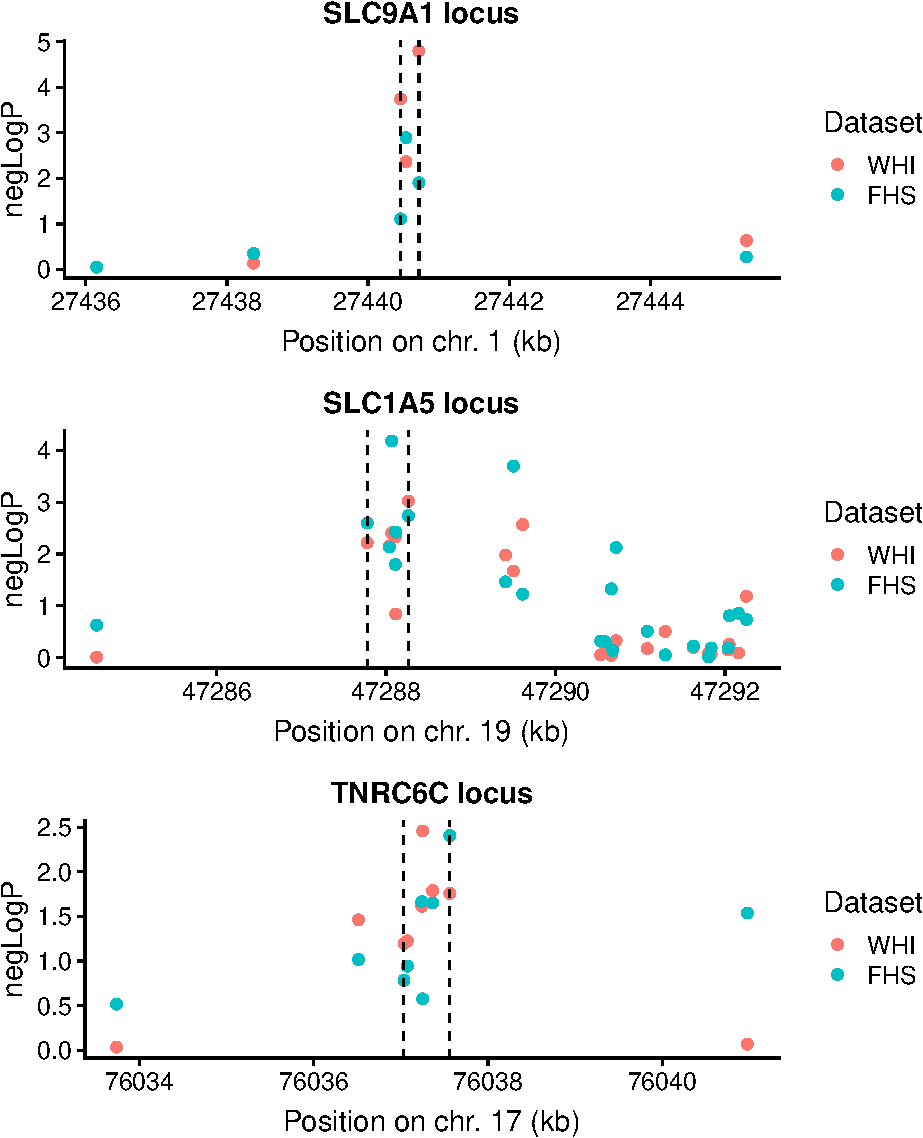
\includegraphics{../doc/figures/combp-plots-1.pdf}
\caption{\label{fig:combp-plots}DMRs identified by Comb-p in WHI and
validated in FHS at the (a) SLC9A1 and (b) SLC1A5 loci. Negative
logarithms of EWAS p-values are shown as a function of the genomic
coordinate. EWAS p-values from WHI are in red and FHS in green. Dotted
lines demarcate the DMR boundaries.}
\end{figure}

\subsection{Exploration of the brown4 and blue
modules}\label{exploration-of-the-brown4-and-blue-modules}

Based on the results from the module- and region-centric analyses, we
investigated the brown4 and blue modules further for biological
significance. The brown4 module was associated with immune-related genes
as noted above, and was enriched strongly for ``open sea'' sites
(p=1.1e-42) and annotated enhancers (p=1.7e-33). In contrast, the blue
module was associated with development-related genes, and was enriched
moderately for sites near genic transcription start sites and strongly
for CpG islands (p \textless{} 2.2e-16) (Fig. 2a,b).

Given these observations, we examined relative enrichments of enhancer-
and promoter-associated histone marks across different blood cell
subtypes to better understand the cell type specificity of this signal.
Epigenetic peaks were annotated using data from the Roadmap Epigenomics
Project (Kundaje et al. 2015) and relative enrichments were calculated
as the fraction of module CpGs found in peaks divided by the fraction of
all CpGs found in peaks. The eFORGE tool is designed to run a similar
cell type specificity analysis, but is currently unable to process CpG
sets the size of the blue module.

We observed the greatest enrichment of brown4 CpGs in
enhancer-associated DNase hypersensitivity sites (DHS) and H3K4me1
histone peaks from monocytes compared to other blood cell subtypes (Fig.
2c). This could point towards monocyte-related biology and inflammatory
processes as an important shared mechanism for cardiovascular risk
between the two cohorts examined here. In contrast, blue CpGs were
enriched for DHS and promoter-associated H3K4me3 histone peaks from
hematopoietic stem cells (HSCs), providing a possible link between
developmental exposures and persistent phenotypic consequences in later
life.

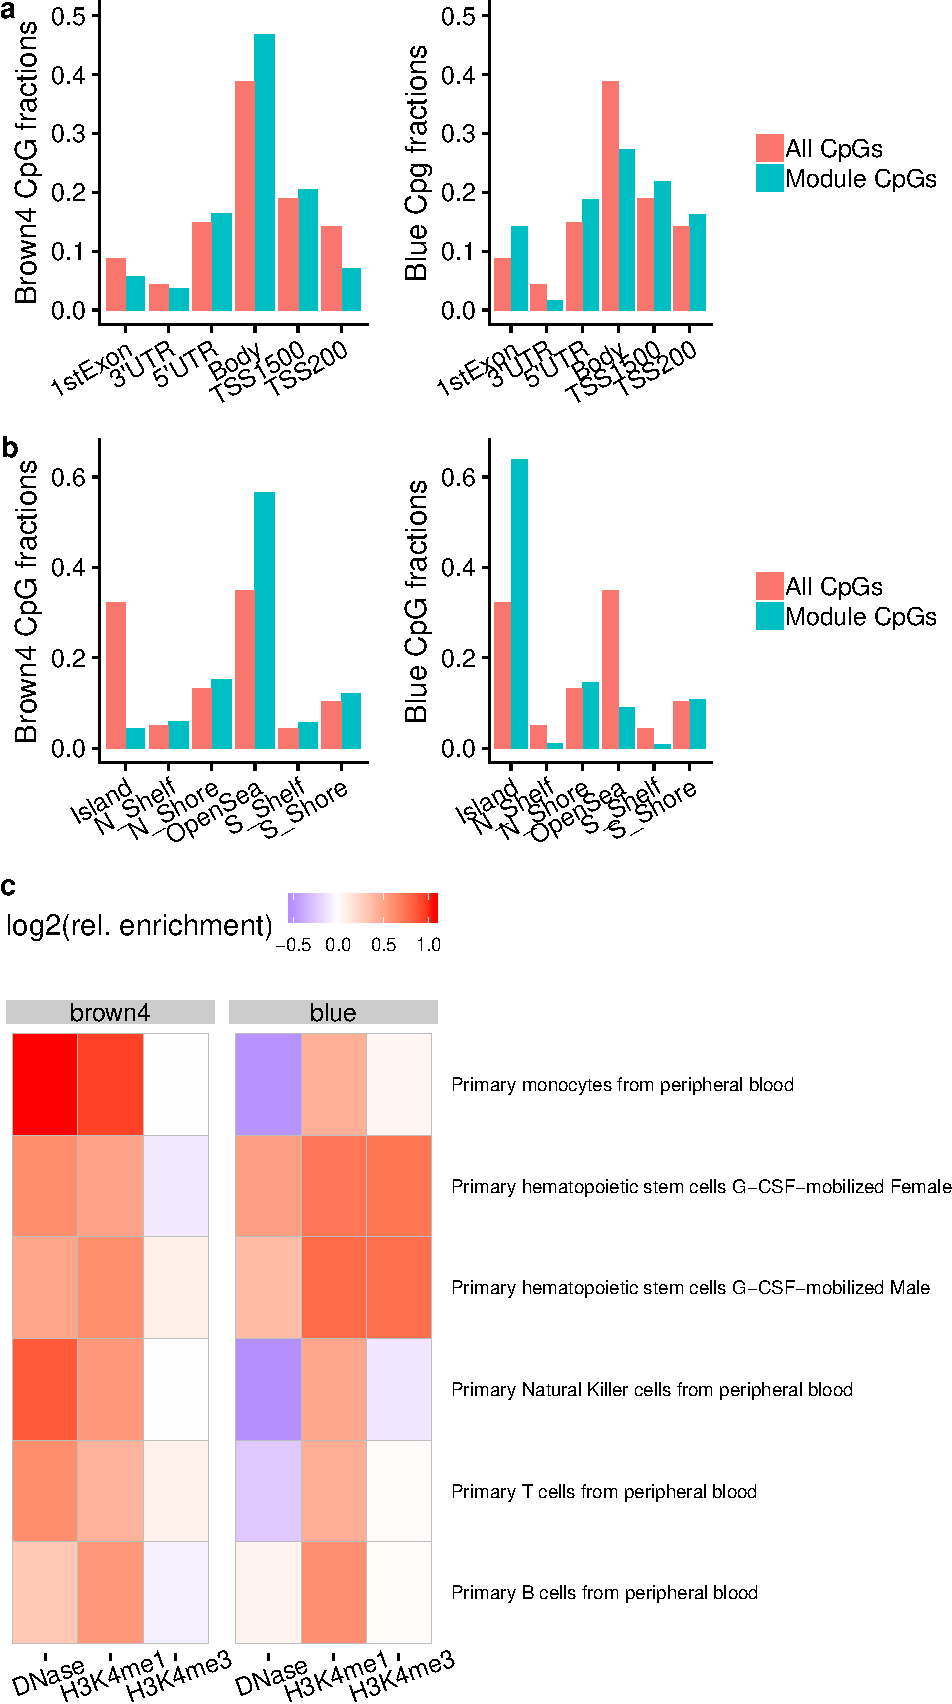
\includegraphics{../doc/figures/brown-and-blue-plots-1.pdf}

The module CpG sets were also compared to two existing methylation-based
age predictors from Horvath and Hannum et al., as well as the recent
morbidity-directed phenoAge(Horvath 2013; Hannum et al. 2013; Levine et
al. 2018). While enrichments for brown4 CpGs were moderate to
nonexistent, blue CpGs were strongly enriched for all three of these
sets, most highly for the original DNAm age developed by Horvath
(34/353; p=1.7e-5; hypergeometric test), despite the fact that this
model was developed based on only \textasciitilde{}21,000 CpGs shared
between multiple versions of the Illumina methylation microarray
platform. Furthermore, 28 of these 34 CpGs had associated positive
coefficients in the DNAm age predictor. This subset has been observed to
contain a disproportionate amount of Polycomb-group target genes, which
are known to associate with both developmental and to be generally
hypermethylated with age(Dozmorov 2015). Surprisingly, the blue eigenCpG
showed only a modest (though statistically significant) correlation with
age (r=0.09).

To find specific genes that may be relevant to the link between blue
module methylation and CVD, a set of genes was assembled constituting
the intersection between 1) genes in one of the top 3 enriched Gene
Ontology terms for the blue module (anatomical development, system
development, and multicellular organism development), 2) genes annotated
to CpGs whose weights in the blue eigenCpG were in the top 10\%, and 3)
genes annotated to environmentally sensitive regions of DNA methylation
in the human embryo as determined by a recent investigation (Kessler et
al. 2018). Exactly one gene, PDE3A, belongs to all three categories.
PDE3A codes for Phosphodiesterase 3A, and as a known gene related to
cardiovascular risk and sensitive to early-life exposures, may represent
one avenue by which the blue module is related to disease risk in adult
life.

\subsection{Module-risk factor
relationships}\label{module-risk-factor-relationships}

\begin{figure}[htbp]
\centering
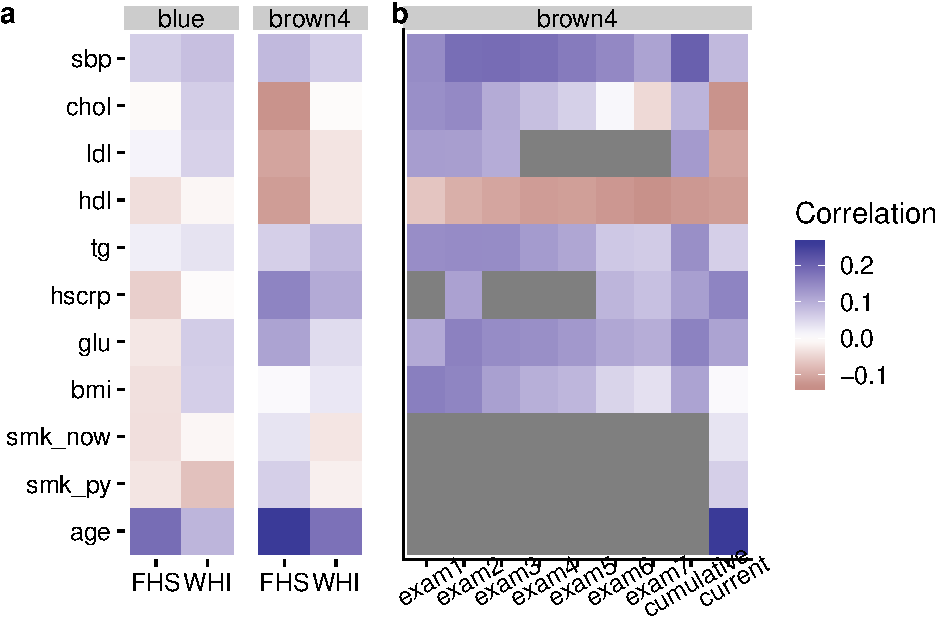
\includegraphics{../doc/figures/risk-factor-correlation-plots-1.pdf}
\caption{\label{fig:risk-factor-correlation-plots}Risk factor-module
relationships. (a) Pearson correlations between a series of traditional
cardiovascular risk factors and module eigenCpGs (blue and brown4) are
shown in each study population. (b) Pearson correlations between
historical risk factor levels in FHS (across previous exams, x-axis) and
current brown4 module activation are shown. Grey panels indicate that
the risk factor in question was not available for the corresponding
exam.}
\end{figure}

Next, we examined correlations between these module eigenCpGs and
traditional cardiovascular risk factors. Though no extremely strong
module-risk factor correlations were observed (all
\textbar{}r\textbar{}\textless{}0.25), they tended to be stronger for
the brown4 module, especially in FHS (Fig. 3a). Age showed the greatest
association, while lipid and glycemic parameters also showed moderate
associations. To further probe relationships between brown4 module and
risk factors in FHS, we retrieved historical risk factors measured in
previous Offspring Cohort exams. Based on visual inspection, there
seemed to be a notably stronger correlation between the module eigenCpG
and cumulative (mean of all previous exams) compared to current risk
factor exposure. This pattern applied for systolic blood pressure
(strongly), triglycerides, glucose, BMI, and LDL (which correlated in
the ``expected'' direction cumulatively, but non-intuitively at Exam 8)
(Fig. 3b).

To better investigate this phenomenon, we tested associations between
the brown4 module and each of the cumulative risk factors after
adjustment for potential confounders. Specifically, for each risk
factor, linear models were used to predict the brown4 eigenCpG value
from either the current or cumulative risk factor level while adjusting
for the full set of EWAS covariates other than BMI (age/sex/smoking/cell
counts/study center/7 ctrl-probe PCs). Only for the brown4 module did
cumulative risk factor exposure show strong associations, which were
generally equal to or stronger than those of the current risk factors,
most notably for BMI, hsCRP, and triglycerides (Table 3). Though more
recent medication use could possibly explain discrepancies between
biological relationships with current and past risk factors, adjustment
for hypertension and lipid medications did not notably affect the
results of these models.

\begin{table}

\caption{\label{tab:cumulative-adjusted}Module-risk factor relationships (current and cumulative) after adjustment for covariates}
\centering
\begin{tabu} to \linewidth {>{\raggedright}X>{\raggedright}X>{\raggedright}X>{\raggedright}X>{\raggedright}X}
\toprule
\multicolumn{1}{c}{} & \multicolumn{2}{c}{brown4} & \multicolumn{2}{c}{blue} \\
\cmidrule(l{2pt}r{2pt}){2-3} \cmidrule(l{2pt}r{2pt}){4-5}
Risk factor & current & cumulative & current & cumulative\\
\midrule
bmi & 0.036 (4.3e-06) & 0.051 (2.3e-10) & 0.026 (0.0061) & 0.019 (0.051)\\
glu & 0.021 (0.011) & 0.027 (0.0011) & -0.00065 (0.95) & -0.0045 (0.66)\\
hscrp & 0.021 (0.0077) & 0.039 (1e-06) & 0.025 (0.011) & 0.014 (0.15)\\
tg & 0.018 (0.02) & 0.042 (5e-07) & 0.021 (0.03) & 0.015 (0.14)\\
hdl & -0.021 (0.015) & -0.017 (0.056) & -0.038 (0.00031) & -0.03 (0.0067)\\
\addlinespace
ldl & -0.012 (0.13) & 0.0089 (0.29) & -0.00072 (0.94) & 0.027 (0.0088)\\
chol & -0.014 (0.11) & 0.019 (0.021) & -0.013 (0.2) & 0.012 (0.24)\\
sbp & 0.012 (0.15) & 0.024 (0.0084) & -0.011 (0.27) & -0.0015 (0.89)\\
\bottomrule
\multicolumn{5}{l}{\textsuperscript{1} Regression results are presented as: beta (p-value).}\\
\multicolumn{5}{l}{\textsuperscript{2} Models are adjusted for age, sex, smoking status and pack-years, estimated cell counts, study center, and 7 control probe principal components.}\\
\end{tabu}
\end{table}

Finally, to assess relationships between cumulative risk factor exposure
and brown4 module activation in predicting cardiovascular risk, we
adopting a causal modeling approach using a series of Cox models in FHS
for these three most strongly-associated risk factors (BMI, hsCRP, and
triglycerides). Covariates in all models included technical factors,
estimated cell counts, age, and sex. Table 5 presents p-values arising
from models incorporating 1) current and cumulative risk factors only,
2) current risk factors and module eigenCpGs only, and 3) all 3
quantities together. As only subjects with current risk factor values
were included in each model, sample sizes were largely identical across
models. In general, the significance of the module relationships with
CVD tended to decrease in the presence of cumulative risk factor values.
This fits with a model in which, rather than mediating cardiovascular
risk, module activation acts as a biomarker for the actions of
cumulative risk factor exposures by some other mechanism.

\begin{table}

\caption{\label{tab:module-mediation}CVD risk models using cumulative risk factor exposure and brown4 module activation}
\centering
\begin{tabular}[t]{llllll}
\toprule
\multicolumn{1}{c}{} & \multicolumn{2}{c}{Risk factors only} & \multicolumn{1}{c}{Brown4 only} & \multicolumn{2}{c}{Full model} \\
\cmidrule(l{2pt}r{2pt}){2-3} \cmidrule(l{2pt}r{2pt}){4-4} \cmidrule(l{2pt}r{2pt}){5-6}
Risk factor & current & cumulative & module & cumulative & module\\
\midrule
bmi & 0.0095 (0.64) & 0.062 (0.008) & 0.013 (0.069) & 0.058 (0.014) & 0.011 (0.12)\\
hscrp & 0.21 (0.15) & 0.65 (<0.001) & 0.015 (0.043) & 0.62 (<0.001) & 0.012 (0.1)\\
tg & 0.34 (0.31) & 1.7 (<0.001) & 0.016 (0.029) & 1.7 (<0.001) & 0.013 (0.082)\\
\bottomrule
\multicolumn{6}{l}{\textsuperscript{1} Regression results are presented as: beta (p-value).}\\
\end{tabular}
\end{table}

\section{Discussion}\label{discussion}

Two of the most important problems facing traditional epigenome-wide
association studies are reverse causation and a lack of reproducibility
of signals at specific loci (Birney, Smith, and Greally 2016). Here, we
addressed these obstacles by performing a primarily module-based
analysis of incident cardiovascular events in order to find prospective
biomarkers and uncover novel mechanisms contributing to disease risk.

We began by constructing correlation-based clusters in the methylation
data from WHI using the WGCNA algorithm. This network-based feature
clustering approach can potentially improve the signal-to-noise ratio of
high-dimensional DNA methylation data while facilitating more clear
biological interpretation of results(Langfelder and Horvath 2008). As
WGCNA does not consider class labels (i.e.~incident CVD status), the 110
modules uncovered were not \emph{a priori} expected to be related to CVD
and rather reflected unbiased patterns in the data. After correction for
multiple testing, the first principal components (eigenCpGs) of three of
these modules were found to be related to incident cardiovascular
events. A gene ontology-based enrichment analysis of the genes annotated
to these modules found strong enrichment for either immune-related or
development-related processes. The finding of immune-related processes
is intuitive given that DNA from blood measures primarily immune cells,
while the development-related enrichment could possibly reflect
influences during early life (Hao et al. 2018). Notably, these two
module ``types'' (immune and development) have been uncovered in a prior
network-based DNA methylation analysis related to asthma (Busch et al.
2016), suggesting that similar module types are a potentially general
feature of blood-based methylation patterns and that these patterns may
not be fully cardiovascular-specific, reflecting instead a
predisposition toward general inflammatory disease processes. Both in
WHI and in replication in FHS, two modules (blue and brown4) showed
strong relationships with incident CVD that were attenuated after
adjustment for age.

We examined the set of module eigenvector loadings as a proxy for the
relative importance of their component CpGs, in a similar approach to
the standard calculation of gene-module correlations (or ``kME''
statistics) in WGCNA analyses. As we did not observe any obvious peaks
distinguishing particularly important groups of CpGs, we undertook an
epigenome-wide association study (EWAS) in order to identify potentially
stronger locus-specific signals. Though we did not find any single sites
replicating in FHS after stringent correction for multiple tests, a
subsequent region-based analysis using the Comb-p algorithm revealed
three regions replicating strongly across the two cohorts examined here.
One was found on chromosome 1 in the body of the SLC9A1 (also known as
NHE-1) gene, which codes for an integral membrane ion transporter
involved in intracellular pH maintenance. It has been shown to be
required for the increased adhesion, migration, and phagocytosis of
oxidized LDL seen in monocytes in response to stimuli including leptin,
adrenaline, and hyperglycemia. Another region discovered was on
chromosome 19 near the transcription start site (TSS) of SLC1A5, which
codes for a neutral amino acid transporter. Though strong evidence does
not yet exist linking SLC1A5 to cardiovascular mechanisms, we note that
its companion amino acid transporter, SLC7A5, is known to regulate
metabolic and inflammatory reprogramming of monocytes in response to
stimulation by lipopolysaccharide (LPS). Notably, CpG sites in both
SLC9A1 and SLC1A5 were discovered and replicated in a recent EWAS for
BMI (including the FHS cohort) {[}Mendelson2017{]}, though that specific
SLC9A1 site was not one of the three constituent CpGs in the region
found here. These two SLC transporter DMRs contained CpGs belonging to
blue (1 in SLC9A1) and brown4 (1 in SLC9A1, 5 in SLC1A5) modules. The
third region was found near the TSS of TNRC6C on chromosome 17. This
gene codes for a component of the miRNA-mediated translational
repression cascade, has shown up in a genome-wide association study
(GWAS) for heart failure (not one of the phenotypes included in our CVD
definition here)(Villard et al. 2011), and was identified as a potential
target gene in the monocyte-to-macrophage transition upon exposure to
CSF-1(Wallner et al. 2016). Common to these three DMRs is a potential
involvement in monocyte biology specific to a stimulus response. This
concept of ``priming'' for subsequent response to stimulus has been
observed with respect to both monocyte activity in CVD (Short et al.
2017) and DNA methylation in general (Lam et al. 2012).

Based on the module- and region-level replication in FHS, we further
explored the characteristics of the brown4 and blue modules. Enrichment
analyses of gene-based and locus-based annotations demonstrated that
these two modules occupy distinct biological niches. Broadly, the brown4
module is enriched for enhancers and other non-proximal regions near
immune-related genes, while the blue module is enriched for CpG islands
near the TSS of development-related genes. One could speculate that
these modules also represent different mechanisms of cardiovascular
risk: one related to inflammatory burden and the other to long-term
effects of early-life exposures, both of which are well-established as
contributing to cardiovascular risk (Nahrendorf 2018; Hao et al. 2018).
Analyses based on cross-tissue epigenome annotations added an additional
dimension to these insights by suggesting differential importance of
blood cell sub-types for these modules. Our custom cell type specificity
analysis, based on the eFORGE algorithm (Breeze et al. 2016), revealed
the enrichment of monocyte-specific regions of open chromatin (DNase
hypersensitivity sites and H3K4me1 peaks) in the brown4 module. This
observation reinforces the idea of monocyte-specific activity suggested
by the replicated DMRs as well as that of ``monocyte priming'' (Short et
al. 2017). Based on the tendency of blue module CpGs to be proximal to
gene TSS, we focused on enrichment for a promoter-associated marker,
H3K4me3, and found a distinct signal related to hematopoietic stem
cells. This finding supports a potential mechanisms linking early-life
exposure to consequences in adult life (Farlik et al. 2016; Laiosa and
Tate 2015).

In seeking a specific example of the mechanism by which the
development-related blue module may by related to CVD risk, we found a
single gene, PDE3A, which is in the blue module's top GO terms, is
annotated to highly-weighted sites in the blue eigenCpG, and is near to
a metastable epiallele found by Kessler et al. to be environmentally
sensitive in developing embryos {[}Kessler2018{]}. PDE3A, encoding for
an isoform of phosphodiesterase 3, has been linked to cardiovascular
disease through its role in regulating vascular smooth muscle cell
contraction. Six missense variants located in PDE3A have been previously
identified as responsible for Mendelian hypertension, and murine models
have suggested that increases in PDE3 activity may mediate some of the
accelerated atherosclerosis observed in diabetes (Maass et al. 2015;
Nagaoka et al. 1998). Interestingly, PDE3A downregulation is potentially
related specifically to heart failure, an outcome that was not included
in our definition of CVD for this study(Yan, Miller, and Abe 2007).

It is not clear whether these methylation modules associate with
cardiovascular risk upstream, downstream, or independently of
traditional cardiovascular risk factors (including age, blood pressure,
BMI, smoking, and lipid levels). To explore these relationships, we
began by calculating correlations between risk factor levels and blue
and brown4 module activations. Blue correlations were largely weak,
while brown4 correlations were somewhat stronger, following the
hypothesis that the blue module is more relevant to early-life, rather
than adult, exposures as compared to brown4. However, as a semi-stable
biological quantity, methylation may have the ability to act as a
``molecular recorder'' of past exposures, ranging from heavy metals to
stress(R. O. Wright et al. 2010; Matosin, Cruceanu, and Binder 2017). We
thus retrieved risk factor measurements from seven prior exams in FHS to
compare ``cumulative'' (calculated as the mean of past exam values)
versus current correlations with brown4 activation. Surprisingly, we
observed stronger correlations with cumulative values across almost all
risk factors. To address the possibility of confounding in these
relationships, we tested linear models predicting brown4 eigenCpG values
from current or cumulative risk factors adjusting for the full set of
EWAS covariates. Here, we again observed multiple instances of stronger
cumulative relationships, especially for BMI, hsCRP, and triglycerides.
Though such a finding could be partially explained by the greater
stability in a mean over seven values compared to one, we note that we
did not observe this same pattern with respect to the blue module, where
associations with current risk factors tended to be stronger. Our
observation agrees with a conceptual model in which known risk factors,
such as the three noted here, act partially through their cumulative
impact over time on immune cell DNA methylation and thus inflammatory
processes known to be related to CVD pathogenesis. To more directly test
this proposal, we used a causal modeling approach in which we
sequentially tested the relationships between cumulative risk factor
levels, brown4 eigenCpG values, and both factors together in predicting
incident CVD. Though neither factor exerted a strong effect on the
relationship of the other, module activation associations were more
weakened after adjustment for cumulative risk factors than the converse.
Thus, our models replicate previous findings that cumulative risk factor
exposure correlates with CVD risk (Reinikainen et al. 2015) while
suggesting that brown4 methylation module activation may be sensing,
rather than mediating, this effect.

A few limitations should be acknowledged in intepreting the results of
this study. First, the observational nature made it impossible to
clearly determine causality of the relationships between methylation and
cardiovascular risk. While the examination of incident CVD reduced
concerns about reverse causation, the discovered associations may only
be markers of other disease-causing processes (such as cumulative risk
factor exposure, as discussed above). Second, assessment of methylation
in blood samples prevented the understanding of potentially causal
epigenetic effects in other CVD-relevant tissues. Although some studies
report promising findings with respect to blood as a proxy tissue(Bacos
et al. 2016), and although development-related epialleles may persist
across tissues, there is a certain gap in our ability to discover
non-blood-related epigenetic patterns in this analysis. Finally,
longitudinal methylation measurements were not available in these
datasets, preventing an analysis of the intra-individual stability of
methylation sites and modules that may be predictive of CVD risk.

The modules and regions discovered in this investigation provide
insights into the complex relationships between DNA methylation and
cardiovascular disease risk. We show that epigenetic modules track with
diverse biological sources of CVD risk, ranging from development- to
immune-related processes, and may provide a molecular readout of past
exposure to cardiovascular risk factors. We further discover specific
differentially methylated regions that may be related to monocyte
activation in response to biological stimuli. This work opens the door
to further investigation of the epigenetic basis of CVD risk as well as
the ability of DNA methylation to act as a biomarker of prior exposures
that may be important for disease-relevant prognosis and interventions.

\section{Methods}\label{methods}

\subsection{Study participants and phenotype
collection}\label{study-participants-and-phenotype-collection}

Data for the discovery set came from a combined case-control and pseudo
case-cohort sampling of 2129 women from the Women's Health Initiative
study, a larger prospective cohort beginning in 1993 that included over
160,000 postmenopausal women from across the United States(Anderson et
al. 1998). Included subjects had no self-reported CVD at baseline, and
cases were chosen based on incident centrally adjudicated angina,
revascularization, or CHD event during follow-up. Inclusion criteria for
methylation measurement resulted in an oversampling of African American
and Hispanic participants. Blood samples used for measurement of DNA
methylation and clinical biochemistry were taken at Exam 1. Data are
available in the dbGaP public repository (accession: phs000200.v11.p3).

Data for the validation set came from a substudy of the Framingham Heart
Study that measured DNA methylation in 2726 subjects from the Offspring
Cohort. The Framingham Offspring Cohort was originally established in
1971 to follow 5209 children of the original Framingham Heart Study
participants and their spouses(Kannel et al. 1979). Fasting blood
samples for both methylation and clinical biochemistry were collected
from participants at Exam 8, which took place from 2005-8. Blood samples
were also provided for clinical biochemistry measurements in previous
exams, constituting the ``past exposures'' examined here. Data are
available in the dbGaP public repository (accession: phs000007.v29.p10).
Adjudicated cardiovascular event data was collected through 2015, and
events were defined here as any of: myocardial infarction, angina
pectoris, stroke, or death from CHD (event codes 1-29).

\subsection{DNA methylation data
processing}\label{dna-methylation-data-processing}

In both cohorts, DNA methylation data were collected using the Illumina
HumanMethylation450 microarray platform(Bibikova et al. 2011).
Preprocessing was performed using the \emph{minfi} and \emph{wateRmelon}
packages for R(Aryee et al. 2014; Pidsley et al. 2013). As a quality
control step, samples were removed if they showed weak overall signal
based on visual inspection of an intensity plot, if they had more than
10\% of probes undetected at a detection threshold of p\textless{}1e-16,
or if the reported sex did not match the predicted sex based on
methylation patterns. Probes were removed if they met any of the
following criteria: more than 10\% of samples undetected at a detection
threshold of p\textless{}1e-16, location in the X or Y chromosomes,
non-CpG probes, cross-hybridizing probes, probes measuring SNPs, and
probes with an annotated SNP at the CpG site or in the single-base
extension region. Samples were normalized using the Noob method for
background correction and dye-bias normalization, followed by the BMIQ
method for probe type correction(Fortin, Triche, and Hansen 2016; A. E.
Teschendorff et al. 2013). For each dataset, principal components
analysis was performed on the set of control probes using code adapted
from the CPACOR method of Lehne et al. to account for technical
variation(Lehne et al. 2015). Blood cell counts for 6 blood cell types
(CD4+ T-cells, CD8+ T-cells, B-cells, natural killer cells, monocytes,
and granulocytes) were estimated using a common reference-based
method(Houseman et al. 2012). After quality control and filtering steps,
422952 (WHI) and 425326 (FHS) CpG sites remained for downstream
analysis, formatted as beta values (ratio of methylated signal to total
microarray signal).

\subsection{Weighted gene correlation network
analysis}\label{weighted-gene-correlation-network-analysis}

Weighted gene correlation network analysis (WGCNA) was used to find
highly correlated modules of CpG sites(B. Zhang and Horvath 2005). The
full set of 422952 CpGs passing quality control from WHI were used as
input. For computational tractability, blockwise module detection was
performed, which treats blocks of features separately for network
creation and module detection, followed by eventual merging of highly
similar modules. To allow for reasonable computation time, the initial
pre-clustering analysis (used to inform the choice of blocks) was
performed in a random subset of 100 subjects. A block size of 20,000 was
used, and a soft-thresholding power of 8 was chosen to balance
approximately scale-free network properties with network connectivity,
Unsigned networks were used, based on the fact that the biological
consequences of an increase vs.~decrease in DNA methylation are much
less clear than those of gene transcripts. Whole-module behavior was
assessed using the first component from a principal components analysis,
performed separately for each module. Scree plots were used to inform
the variance explained by each module as well as to justify the use of a
single eigenvector as a proxy for module behavior. Module preservation
assessment in was completed in FHS, resulting in \(Z_{summary}\)
statistics to confirm cross-dataset robustness of module
connectivity(Langfelder et al. 2011). EigenCpGs were then calculated
(according to the principal component weights from WHI), followed by
assessment of associations with incident CVD.

Module associations with cardiovascular disease were assessed using Cox
proportional hazards regressions, with eigenCpGs as the independent
variable and time-to-event measures for incident CVD as the dependent
variable. Minimal models adjusted for estimated blood cell counts as
well as technical covariates (DNA pull batch in WHI; analysis center + 7
control-probe principal components in FHS -- see EWAS section for
details). Fully-adjusted models adjusted additionally for biological
covariates (age, bmi, smoking status, and pack-years of smoking; sex in
FHS; race in WHI).

\subsection{Epigenome-wide associations of DNA methylation with incident
CVD
events}\label{epigenome-wide-associations-of-dna-methylation-with-incident-cvd-events}

For the EWAS analysis, each CpG site was assessed using the the same
regression framework as in the module-based models, separately in both
WHI and FHS. Methylation beta-values replaced eigenCpGs as the
independent variable, and the full set of technical and biological
covariates was used. To remove the influence of beta-value outliers,
samples were excluded for each CpG if their beta value was outside of
the ``outer fence'' (\textless{} 25\%ile - \(3*IQR\) or \textgreater{}
75\%ile + \(3*IQR\)). QQ plots and calculation of the genomic inflation
factor \(\lambda\) revealed that genomic inflation was not adequately
controlled in FHS, so 7 CPACOR principal components (chosen based on a
Scree plot assessment of CPACOR results) were additionally adjusted for
in FHS. CPACOR uses principal components analysis on the set of control
probes from the methylation array in order to estimate and control for
potential batch effects without disturbing biological signal (Lehne et
al. 2015). Proportional hazards checks were implemented (cox.zph
function in R) for the top EWAS hits in WHI, and no systematic departure
from the Cox regression assumptions were detected.

Comb-p, implemented as a Python module, was used to call differentially
methylated regions (DMRs). The algorithm takes as input p-values from
the EWAS, removing the requirement for additional covariate adjustment.
Comb-p first calculates an autocorrelation function (ACF), for which a
maximum distance of 1kb and a step size of 50 bases were used. Next, it
uses the ACF to adjust each p-value using a Stouffer-Liptak-Kechris
correction, followed by identification of contiguous regions of sites
with adjusted p-values below some threshold (here, p\textless{}0.1 with
no more than 500 bases between neighboring sites in a region). Finally,
the ACF is recalculated out to the maximum region size (a step size of
50 was used here as well) and regional p-values are calculated using the
Stouffer-Liptak test. For multiple testing correction of DMRs, Comb-p
calculates the number of effective tests separately for each DMR as the
number of loci tested divided by the size of the region (typically
\textasciitilde{}1kb).

\subsection{Module enrichment
analyses}\label{module-enrichment-analyses}

Gene ontology-based enrichment analysis of DMPs was performed using the
gometh function from the \emph{missMethyl} package for R. In this
procedure, gene annotations for CpG sites are retrieved, and enrichment
analysis is performed while accounting for the bias in number of CpG
probes per gene on the microarray.

Locus-based enrichment analyses were performed using basic two-tailed
hypergeometric tests for overlap between module membership and
annotation category membership. CpG annotations with respect to both CpG
islands (Island, North shore, Open sea, etc.) and genes (TSS1500, 3'
UTR, Body, etc.) were retrieved from the standard Illumina
HumanMethylation450 microarray annotation.

\subsection{Inference of cell type
specificity}\label{inference-of-cell-type-specificity}

Epigenomic annotations were used to test for relative enrichment of
module CpGs in cell type-specific regulatory regions. Annotations for
broad peaks in DNase sensitivity as well as ChIP-seq signal for H3K4me1
and H3K4me3 were obtained for 6 blood cell types (monocytes, natural
killer cells, T-cells, B-cells, and hematopoietic stems cells from males
and females) from the NIH Roadmap Epigenomics Project database (Kundaje
et al. 2015). For each combination of epigenomic feature and cell type,
CpGs from the HumanMethylation450 array were classified as to their
membership in a peak region. Relative enrichments of in-peak CpGs for
modules were then calculated as the ratio of
\(\frac{\#CpG_{in-peak}}{\#CpG_{total}}_{module}\) to
\(\frac{\#CpG_{in-peak}}{\#CpG_{total}}_{all}\) and presented as
\(log_2\)(relative enrichment) for ease of visualization. Cell type
specificity of different modules can then be compared by examining
relative enrichments across cell types, especially with respect to
highly-represented regulatory annotation types (e.g.~DNase
hypersensitivity sites for a module enriched in enhancers). We note that
this method borrows from the permutation-based eFORGE tool methodology
(Breeze et al. 2016), which could not be used here due to the size of
the blue module.

\subsection{Risk factor integration}\label{risk-factor-integration}

Risk factors were incorporated into the module-based analysis in a
series of steps. First, Pearson correlations between risk factor levels
and module eigenCpGs were calculated to provide a high-level
understanding of the strength of their relationship. Risk factors in WHI
were all measured at Exam 1 (concurrently with the methylation
measurement), while risk factors in FHS were collected for all exams
prior to and including Exam 8 (the time of the methylation measurement).
In FHS, correlations with past risk factor levels as well as a
``cumulative'' exposure level (equal to the mean of each set of risk
factor levels from Exam 1-7) were also calculated.

Next, linear models were used to assess these same module-risk factor
correlations in FHS while adjusting for potential confounding variables.
These models predicted module eigenCpGs using either cumulative (Exams
1-7) or current (Exam 8) risk factors, while adjusting for the same set
of technical and biological covariates as in the EWAS (described above).
In this step, both eigenCpGs and risk factors were standardized before
modeling in order to facilitate effect size comparisons across risk
factors and across modules.

Finally, the relationship between cumulative risk factors, the brown4
module, and incident CVD was examined using the same Cox regression
setup as in the EWAS. This component involved three subsequent models,
all adjusting for the full set of technical and biological covariates as
well as the ``current'' level of the risk factor in question: the first
using only cumulative risk factors, the second using only the brown4
eigenCpG, and the third using both simultaneously.

\newpage

\section{Supplementary}\label{supplementary}

\newcommand{\beginsupplement}{
  \setcounter{table}{0}  
  \renewcommand{\thetable}{S\arabic{table}} 
  \setcounter{figure}{0} 
  \renewcommand{\thefigure}{S\arabic{figure}}
}

\beginsupplement

\begin{figure}[htbp]
\centering
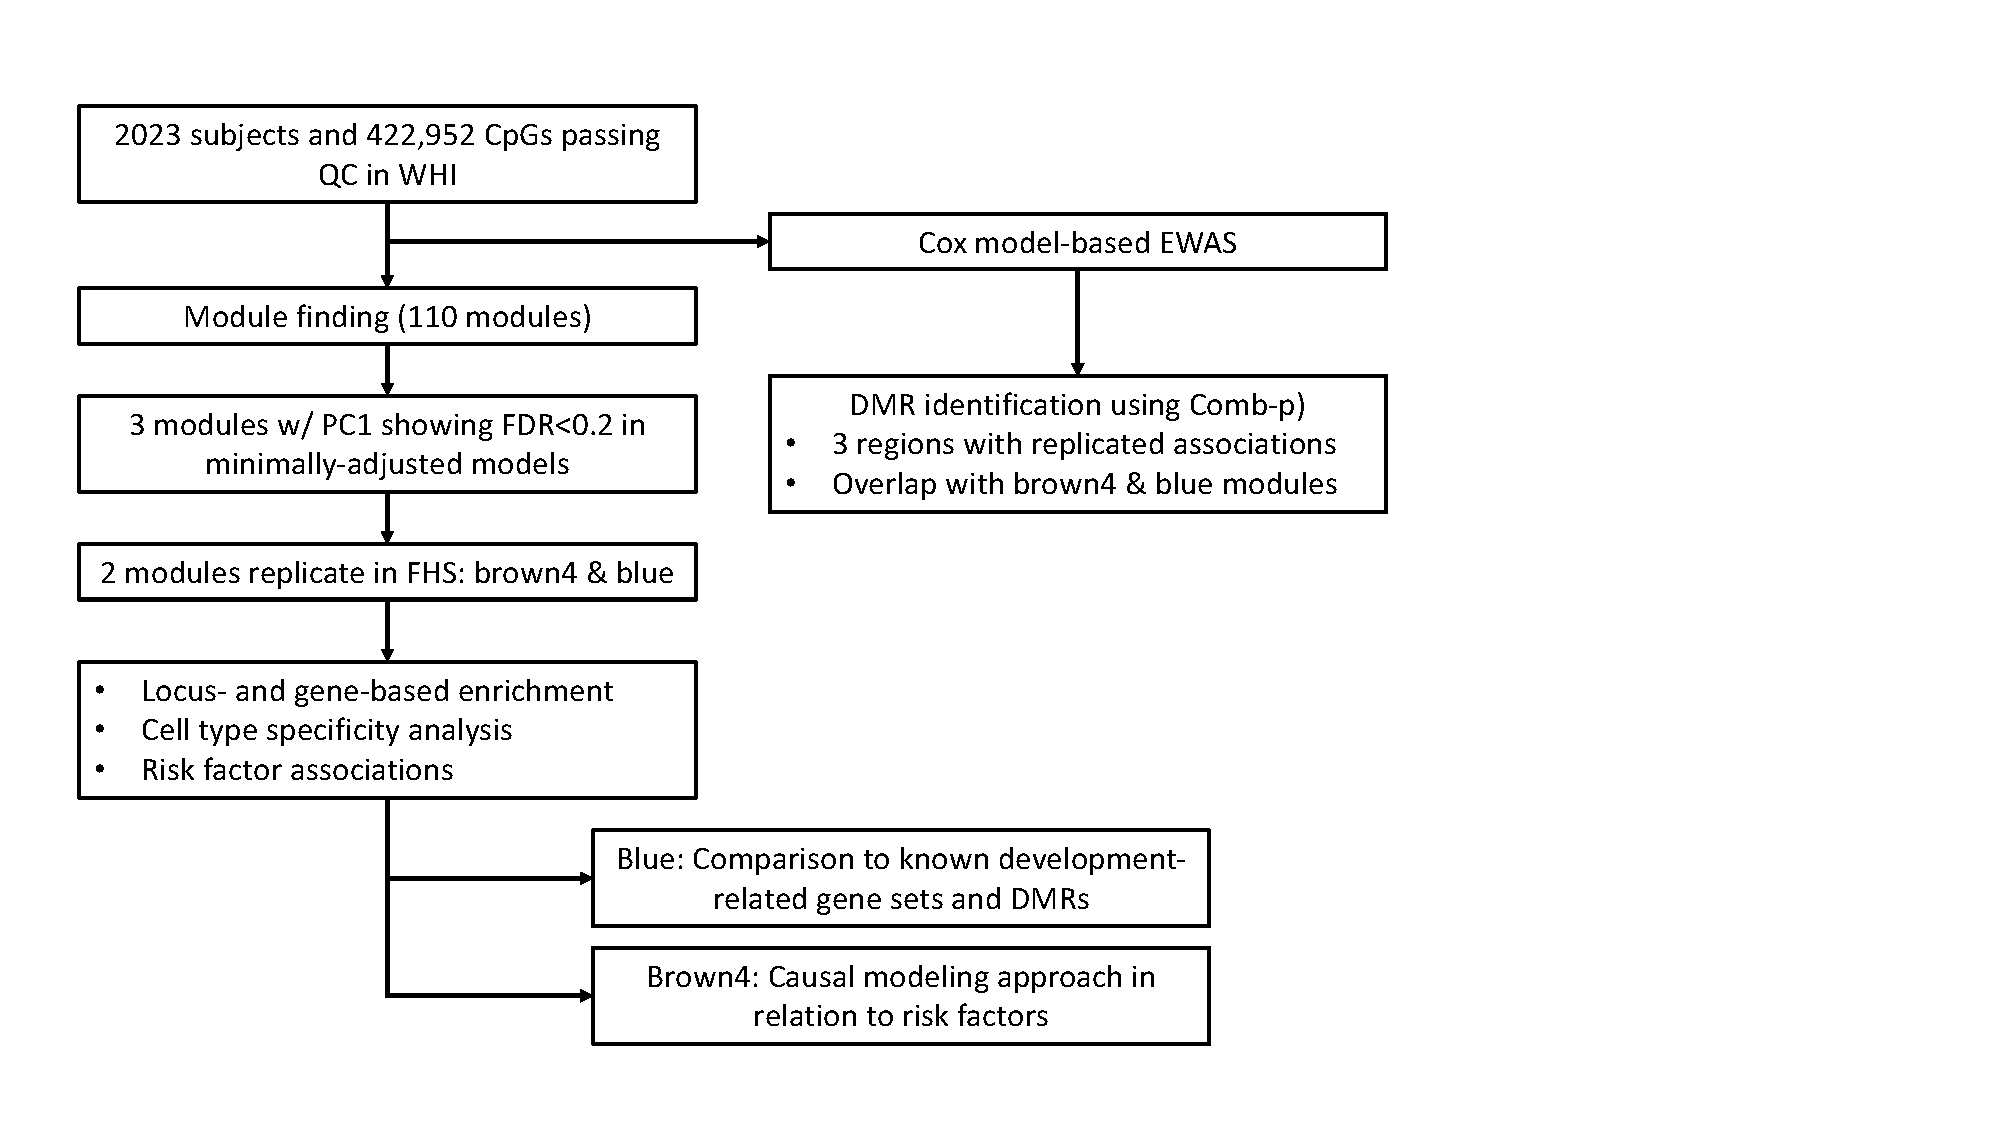
\includegraphics{../doc/figures/workflow.pdf}
\caption{\label{fig:workflow}Study overview, including module- and
region-based analyses as well as follow-up.}
\end{figure}

\begin{figure}[htbp]
\centering
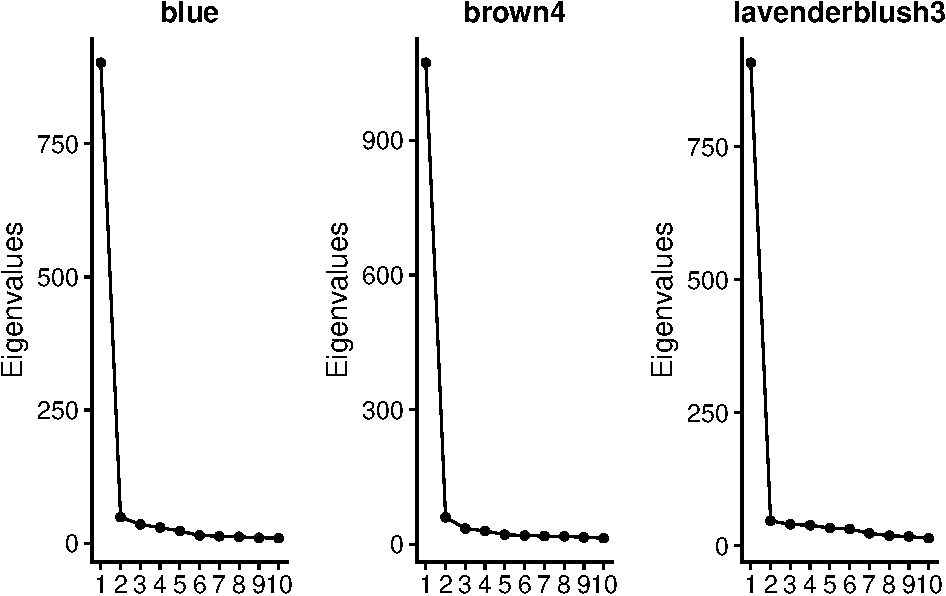
\includegraphics{../doc/figures/print-scree-plots-1.pdf}
\caption{\label{fig:print-scree-plots}Scree plots for PCA on the set of CpGs
corresponding to each of the top modules.}
\end{figure}

\begin{tabular}{lrrrr}
\toprule
\multicolumn{1}{c}{} & \multicolumn{2}{c}{WHI (discovery)} & \multicolumn{2}{c}{FHS (replication)} \\
\cmidrule(l{2pt}r{2pt}){2-3} \cmidrule(l{2pt}r{2pt}){4-5}
Module & Partially adjusted & Fully adjusted & Partially adjusted & Fully adjusted\\
\midrule
blue & 0.0002736 & 0.0500018 & 0.0000085 & 0.8189348\\
brown4 & 0.0045462 & 0.0872688 & 0.0000962 & 0.0997390\\
lavenderblush3 & 0.0050028 & 0.0210976 & 0.0202819 & 0.1580861\\
\bottomrule
\multicolumn{5}{l}{\textsuperscript{1} Partially-adjusted models are adjusted for technical covariates (DNA pull batch in WHI and study center + 7 control probe PCs in FHS) and estimated cell counts. Fully-adjusted models are additionally adjusted for age, sex, smoking status and smoking pack-years.}\\
\end{tabular}

\begin{table}

\caption{\label{tab:ewas-cpgs}CpGs with FDR<0.05 in the discovery set (Bonferroni threshold = 1.18e-7)}
\centering
\begin{tabular}[t]{lllllll}
\toprule
CpG & Chromosome & Direction of Association & P-value & Location & Annotated Gene & Replication P-value\\
\midrule
cg09155044 & chr16 & + & 6.63e-09 & TSS1500 & VKORC1 & 0.107\\
cg24434800 & chr1 & + & 5.04e-08 &  &  & 0.629\\
cg11691298 & chr2 & + & 1.1e-07 & Body & FAM59B & 0.525\\
cg02379107 & chr20 & + & 4.72e-07 & TSS1500 & KIAA1755 & 0.930\\
\bottomrule
\end{tabular}
\end{table}

\begin{figure}[htbp]
\centering
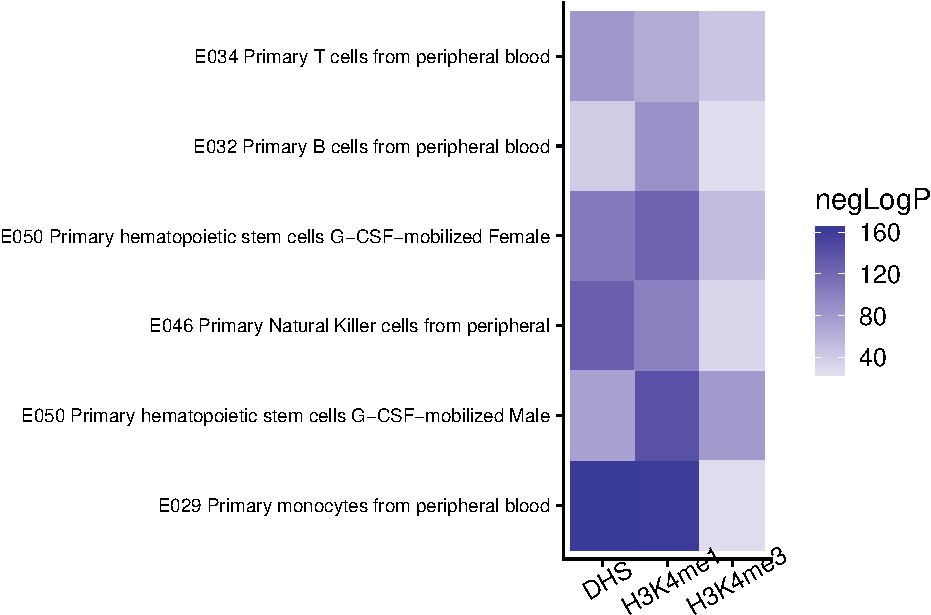
\includegraphics{../doc/figures/print-eforge-plots-1.pdf}
\caption{\label{fig:print-eforge-plots}eFORGE cell type-specificity plot for
the brown4 module.}
\end{figure}

\section*{References}\label{references}
\addcontentsline{toc}{section}{References}

Anderson, Garnet L, Steven R Cummings, Laurence S Freedman, Curt
Furberg, Maureen M Henderson, Susan R Johnson, Lewis H Kuller, et al.
1998. ``Design of the Women's Health Initiative Clinical Trial and
Observational Study.'' \emph{Controlled Clinical Trials} 19 (1):
61--109.
doi:\href{http://dx.doi.org/10.1016/S0197-2456(97)00078-0}{10.1016/S0197-2456(97)00078-0}.

Aryee, Martin J., Andrew E. Jaffe, Hector Corrada-Bravo, Christine
Ladd-Acosta, Andrew P. Feinberg, Kasper D. Hansen, and Rafael A.
Irizarry. 2014. ``Minfi: A flexible and comprehensive Bioconductor
package for the analysis of Infinium DNA methylation microarrays.''
\emph{Bioinformatics} 30 (10). Oxford University Press: 1363--69.
doi:\href{http://dx.doi.org/10.1093/bioinformatics/btu049}{10.1093/bioinformatics/btu049}.

Aslibekyan, Stella, Golareh Agha, Elena Colicino, Anh N. Do, Jari Lahti,
Symen Ligthart, Riccardo E. Marioni, et al. 2018. ``Association of
Methylation Signals With Incident Coronary Heart Disease in an
Epigenome-Wide Assessment of Circulating Tumor Necrosis Factor
\(\alpha\).'' \emph{JAMA Cardiology} 3 (6): 463--72.
doi:\href{http://dx.doi.org/10.1001/JAMACARDIO.2018.0510}{10.1001/JAMACARDIO.2018.0510}.

Baccarelli, A, R Wright, V Bollati, A Litonjua, A Zanobetti, L
Tarantini, D Sparrow, P Vokonas, and J Schwartz. 2010. ``Ischemic heart
disease and stroke in relation to blood DNA methylation.''
\emph{Epidemiology} 21 (6): 819--28.
doi:\href{http://dx.doi.org/10.1097/EDE.0b013e3181f20457}{10.1097/EDE.0b013e3181f20457}.

Bacos, Karl, Linn Gillberg, Petr Volkov, Anders H Olsson, Torben Hansen,
Oluf Pedersen, Anette Prior Gjesing, et al. 2016. ``Blood-based
biomarkers of age-associated epigenetic changes in human islets
associate with insulin secretion and diabetes.'' \emph{Nature
Communications} 7. Nature Publishing Group: 11089.
doi:\href{http://dx.doi.org/10.1038/ncomms11089}{10.1038/ncomms11089}.

B{ä}ck, Magnus, and G{ö}ran K. Hansson. 2015. ``Anti-inflammatory
therapies for atherosclerosis.'' \emph{Nature Reviews Cardiology}.
doi:\href{http://dx.doi.org/10.1038/nrcardio.2015.5}{10.1038/nrcardio.2015.5}.

Bibikova, Marina, Bret Barnes, Chan Tsan, Vincent Ho, Brandy Klotzle,
Jennie M. Le, David Delano, et al. 2011. ``High density DNA methylation
array with single CpG site resolution.'' \emph{Genomics} 98 (4):
288--95.
doi:\href{http://dx.doi.org/10.1016/j.ygeno.2011.07.007}{10.1016/j.ygeno.2011.07.007}.

Birney, Ewan, George Davey Smith, and John M Greally. 2016.
``Epigenome-wide Association Studies and the Interpretation of Disease
-Omics.'' Edited by Gregory S. Barsh. \emph{PLOS Genetics} 12 (6):
e1006105.
doi:\href{http://dx.doi.org/10.1371/journal.pgen.1006105}{10.1371/journal.pgen.1006105}.

Bonder, Marc Jan, Ren{é} Luijk, Daria V Zhernakova, Matthijs Moed,
Patrick Deelen, Martijn Vermaat, Maarten van Iterson, et al. 2016.
``Disease variants alter transcription factor levels and methylation of
their binding sites.'' \emph{Nature Genetics} 49 (1): 131--38.
doi:\href{http://dx.doi.org/10.1038/ng.3721}{10.1038/ng.3721}.

Breeze, Charles E., Dirk S. Paul, Jenny van Dongen, Lee M. Butcher, John
C. Ambrose, James E. Barrett, Robert Lowe, et al. 2016. ``eFORGE: A Tool
for Identifying Cell Type-Specific Signal in Epigenomic Data.''
\emph{Cell Reports} 17 (8). Cell Press: 2137--50.
doi:\href{http://dx.doi.org/10.1016/j.celrep.2016.10.059}{10.1016/j.celrep.2016.10.059}.

Busch, Robert, Weiliang Qiu, Jessica Lasky-Su, Jarrett Morrow, Gerard
Criner, and Dawn DeMeo. 2016. ``Differential DNA methylation marks and
gene comethylation of COPD in African-Americans with COPD
exacerbations.'' \emph{Respiratory Research} 17 (1): 143.
doi:\href{http://dx.doi.org/10.1186/s12931-016-0459-8}{10.1186/s12931-016-0459-8}.

Dekkers, Koen F, Maarten van Iterson, Roderick C Slieker, Matthijs H
Moed, Marc Jan Bonder, Michiel van Galen, Hailiang Mei, et al. 2016.
``Blood lipids influence DNA methylation in circulating cells.''
\emph{Genome Biology} 17 (1): 138.
doi:\href{http://dx.doi.org/10.1186/s13059-016-1000-6}{10.1186/s13059-016-1000-6}.

Dozmorov, Mikhail G. 2015. ``Polycomb repressive complex 2 epigenomic
signature defines age-associated hypermethylation and gene expression
changes.'' \emph{Epigenetics} 10 (6). Taylor \& Francis: 484--95.
doi:\href{http://dx.doi.org/10.1080/15592294.2015.1040619}{10.1080/15592294.2015.1040619}.

Farlik, Matthias, Florian Halbritter, Fabian M{ü}ller, Fizzah A Choudry,
Peter Ebert, Johanna Klughammer, Samantha Farrow, et al. 2016. ``DNA
Methylation Dynamics of Human Hematopoietic Stem Cell Differentiation.''
\emph{Cell Stem Cell} 19 (6). Elsevier: 808--22.
doi:\href{http://dx.doi.org/10.1016/j.stem.2016.10.019}{10.1016/j.stem.2016.10.019}.

Fern{á}ndez-Sanl{é}s, Alba, Sergi Sayols-Baixeras, Isaac Subirana, Irene
R Degano, and Roberto Elosua. 2017. ``Association between DNA
methylation and coronary heart disease or other atherosclerotic events:
A systematic review.'' \emph{Atherosclerosis}.
doi:\href{http://dx.doi.org/10.1016/j.atherosclerosis.2017.05.022}{10.1016/j.atherosclerosis.2017.05.022}.

Fortin, Jean-Philippe, Timothy J Triche, and Kasper D Hansen. 2016.
``Preprocessing, normalization and integration of the Illumina
HumanMethylationEPIC array with minfi.'' \emph{Bioinformatics} 33 (4).
Oxford University Press: btw691.
doi:\href{http://dx.doi.org/10.1093/bioinformatics/btw691}{10.1093/bioinformatics/btw691}.

Guarrera, Simonetta, Giovanni Fiorito, N Charlotte Onland-Moret, Alessia
Russo, Claudia Agnoli, Alessandra Allione, Cornelia {Di Gaetano}, et al.
2015. ``Gene-specific DNA methylation profiles and LINE-1
hypomethylation are associated with myocardial infarction risk.''
\emph{Clinical Epigenetics} 7 (1): 133.
doi:\href{http://dx.doi.org/10.1186/s13148-015-0164-3}{10.1186/s13148-015-0164-3}.

Hannum, Gregory, Justin Guinney, Ling Zhao, Li Zhang, Guy Hughes,
Srinivas Sadda, Brandy Klotzle, et al. 2013. ``Genome-wide Methylation
Profiles Reveal Quantitative Views of Human Aging Rates.''
\emph{Molecular Cell} 49 (2): 359--67.
doi:\href{http://dx.doi.org/10.1016/j.molcel.2012.10.016}{10.1016/j.molcel.2012.10.016}.

Hao, Guang, Nagy A. Youssef, Catherine L. Davis, and Shaoyong Su. 2018.
``The role of DNA methylation in the association between childhood
adversity and cardiometabolic disease.'' \emph{International Journal of
Cardiology} 255 (March). Elsevier: 168--74.
doi:\href{http://dx.doi.org/10.1016/j.ijcard.2017.12.063}{10.1016/j.ijcard.2017.12.063}.

Hedman, {Å}sa K., Michael M. Mendelson, Riccardo E. Marioni, Stefan
Gustafsson, Roby Joehanes, Marguerite R. Irvin, Degui Zhi, et al. 2017.
``Epigenetic Patterns in Blood Associated With Lipid Traits Predict
Incident Coronary Heart Disease Events and Are Enriched for Results From
Genome-Wide Association Studies.'' \emph{Circulation: Cardiovascular
Genetics} 10 (1): e001487.
doi:\href{http://dx.doi.org/10.1161/CIRCGENETICS.116.001487}{10.1161/CIRCGENETICS.116.001487}.

Horvath, Steve. 2013. ``DNA methylation age of human tissues and cell
types.'' \emph{Genome Biology} 14 (10): R115.
doi:\href{http://dx.doi.org/10.1186/gb-2013-14-10-r115}{10.1186/gb-2013-14-10-r115}.

Houseman, Eugene Andres, William P Accomando, Devin C Koestler, Brock C
Christensen, Carmen J Marsit, Heather H Nelson, John K Wiencke, and Karl
T Kelsey. 2012. ``DNA methylation arrays as surrogate measures of cell
mixture distribution.'' \emph{BMC Bioinformatics} 13 (1): 86.
doi:\href{http://dx.doi.org/10.1186/1471-2105-13-86}{10.1186/1471-2105-13-86}.

Huang, Yen Tsung, Su Chu, Eric B Loucks, Chien Ling Lin, Charles B
Eaton, Stephen L Buka, and Karl T Kelsey. 2016. ``Epigenome-wide
profiling of DNA methylation in paired samples of adipose tissue and
blood.'' \emph{Epigenetics} 11 (3): 227--36.
doi:\href{http://dx.doi.org/10.1080/15592294.2016.1146853}{10.1080/15592294.2016.1146853}.

Irvin, Marguerite R., Degui Zhi, Roby Joehanes, Michael Mendelson,
Stella Aslibekyan, Steven A. Claas, Krista S. Thibeault, et al. 2014.
``Epigenome-wide association study of fasting blood lipids in the
genetics of lipid-lowering drugs and diet network study.''
\emph{Circulation} 130 (7): 565--72.
doi:\href{http://dx.doi.org/10.1161/CIRCULATIONAHA.114.009158}{10.1161/CIRCULATIONAHA.114.009158}.

Kannel, William B, Manning Feinleib, Patricia M. Mcnamara, Robert J
Garrison, and William P Castelli. 1979. ``An investigation of coronary
heart disease in families: The framingham offspring study.''
\emph{American Journal of Epidemiology} 110 (3): 281--90.
doi:\href{http://dx.doi.org/10.1093/oxfordjournals.aje.a112813}{10.1093/oxfordjournals.aje.a112813}.

Kessler, Noah J., Robert A. Waterland, Andrew M. Prentice, and Matt J.
Silver. 2018. ``Establishment of environmentally sensitive DNA
methylation states in the very early human embryo.'' \emph{Science
Advances} 4 (7). American Association for the Advancement of Science:
eaat2624.
doi:\href{http://dx.doi.org/10.1126/sciadv.aat2624}{10.1126/sciadv.aat2624}.

Kundaje, Anshul, Wouter Meuleman, Jason Ernst, Misha Bilenky, Angela
Yen, Alireza Heravi-Moussavi, Pouya Kheradpour, et al. 2015.
``Integrative analysis of 111 reference human epigenomes.''
\emph{Nature} 518 (7539): 317--30.
doi:\href{http://dx.doi.org/10.1038/nature14248}{10.1038/nature14248}.

Laiosa, Michael D., and Everett R. Tate. 2015. ``Fetal Hematopoietic
Stem Cells Are the Canaries in the Coal Mine That Portend Later Life
Immune Deficiency.'' \emph{Endocrinology} 156 (10). Oxford University
Press: 3458--65.
doi:\href{http://dx.doi.org/10.1210/en.2015-1347}{10.1210/en.2015-1347}.

Lam, Lucia L, Eldon Emberly, Hunter B Fraser, Sarah M Neumann, Edith
Chen, Gregory E Miller, and Michael S Kobor. 2012. ``Factors underlying
variable DNA methylation in a human community cohort.''
\emph{Proceedings of the National Academy of Sciences} 109
(Supplement\_2): 17253--60.
doi:\href{http://dx.doi.org/10.1073/pnas.1121249109}{10.1073/pnas.1121249109}.

Langfelder, Peter, and Steve Horvath. 2008. ``WGCNA: An R package for
weighted correlation network analysis.'' \emph{BMC Bioinformatics} 9.
doi:\href{http://dx.doi.org/10.1186/1471-2105-9-559}{10.1186/1471-2105-9-559}.

Langfelder, Peter, Rui Luo, Michael C Oldham, and Steve Horvath. 2011.
``Is My Network Module Preserved and Reproducible?'' Edited by Philip E.
Bourne. \emph{PLoS Computational Biology} 7 (1). Public Library of
Science: e1001057.
doi:\href{http://dx.doi.org/10.1371/journal.pcbi.1001057}{10.1371/journal.pcbi.1001057}.

Lehne, Benjamin, Alexander W. Drong, Marie Loh, Weihua Zhang, William R.
Scott, Sian Tsung Tan, Uzma Afzal, et al. 2015. ``A coherent approach
for analysis of the Illumina HumanMethylation450 BeadChip improves data
quality and performance in epigenome-wide association studies.''
\emph{Genome Biology} 16 (1).
doi:\href{http://dx.doi.org/10.1186/s13059-015-0600-x}{10.1186/s13059-015-0600-x}.

Levine, Morgan E., Ake T. Lu, Austin Quach, Brian H. Chen, Themistocles
L. Assimes, Stefania Bandinelli, Lifang Hou, et al. 2018. ``An
epigenetic biomarker of aging for lifespan and healthspan.''
\emph{Aging} 10 (4): 573--91.
doi:\href{http://dx.doi.org/10.18632/aging.101414}{10.18632/aging.101414}.

Li, Jun, Xiaoyan Zhu, Kuai Yu, Haijing Jiang, Yizhi Zhang, Siyun Deng,
Longxian Cheng, et al. 2017. ``Genome-Wide Analysis of DNA Methylation
and Acute Coronary Syndrome.'' \emph{Circulation Research} 120 (11):
1754--67.
doi:\href{http://dx.doi.org/10.1161/CIRCRESAHA.116.310324}{10.1161/CIRCRESAHA.116.310324}.

Maass, Philipp G, Atakan Aydin, Friedrich C Luft, Carolin Sch{ä}chterle,
Anja Weise, Sigmar Stricker, Carsten Lindschau, et al. 2015. ``PDE3A
mutations cause autosomal dominant hypertension with brachydactyly.''
\emph{Nature Genetics} 47 (6): 647--53.
doi:\href{http://dx.doi.org/10.1038/ng.3302}{10.1038/ng.3302}.

Matosin, Natalie, Cristiana Cruceanu, and Elisabeth B Binder. 2017.
``Preclinical and Clinical Evidence of DNA Methylation Changes in
Response to Trauma and Chronic Stress.'' \emph{Chronic Stress} 1
(January): 247054701771076.
doi:\href{http://dx.doi.org/10.1177/2470547017710764}{10.1177/2470547017710764}.

Nagaoka, Tadasu, Taku Shirakawa, Thomas W Balon, James C Russell, and
Yoko Fujita-Yamaguchi. 1998. ``Cyclic nucleotide phosphodiesterase 3
expression in vivo: Evidence for tissue-specific expression of
phosphodiesterase 3A or 3B mRNA and activity in the aorta and adipose
tissue of atherosclerosis-prone insulin-resistant rats.''
\emph{Diabetes} 47 (7): 1135--44.
doi:\href{http://dx.doi.org/10.2337/diabetes.47.7.1135}{10.2337/diabetes.47.7.1135}.

Nahrendorf, Matthias. 2018. ``Myeloid cell contributions to
cardiovascular health and disease.'' \emph{Nature Medicine}.
doi:\href{http://dx.doi.org/10.1038/s41591-018-0064-0}{10.1038/s41591-018-0064-0}.

Nakatochi, Masahiro, Sahoko Ichihara, Ken Yamamoto, Keiko Naruse,
Shigeki Yokota, Hiroyuki Asano, Tatsuaki Matsubara, and Mitsuhiro
Yokota. 2017. ``Epigenome-wide association of myocardial infarction with
DNA methylation sites at loci related to cardiovascular disease.''
\emph{Clinical Epigenetics} 9 (1).
doi:\href{http://dx.doi.org/10.1186/s13148-017-0353-3}{10.1186/s13148-017-0353-3}.

Ordov{á}s, Jos{é} M., and Caren E. Smith. 2010. ``Epigenetics and
cardiovascular disease.'' \emph{Nature Reviews Cardiology} 7 (9):
510--19.
doi:\href{http://dx.doi.org/10.1038/nrcardio.2010.104}{10.1038/nrcardio.2010.104}.

Pfeiffer, Liliane, Simone Wahl, Luke C. Pilling, Eva Reischl, Johanna K.
Sandling, Sonja Kunze, Lesca M. Holdt, et al. 2015. ``DNA Methylation of
Lipid-Related Genes Affects Blood Lipid Levels.'' \emph{Circulation:
Cardiovascular Genetics} 8 (2): 334--42.
doi:\href{http://dx.doi.org/10.1161/CIRCGENETICS.114.000804}{10.1161/CIRCGENETICS.114.000804}.

Pidsley, Ruth, Chloe C {Y Wong}, Manuela Volta, Katie Lunnon, Jonathan
Mill, and Leonard C Schalkwyk. 2013. ``A data-driven approach to
preprocessing Illumina 450K methylation array data.'' \emph{BMC
Genomics} 14 (1). BioMed Central: 293.
doi:\href{http://dx.doi.org/10.1186/1471-2164-14-293}{10.1186/1471-2164-14-293}.

Rask-Andersen, Mathias, David Martinsson, Muhammad Ahsan, Stefan Enroth,
Weronica E Ek, Ulf Gyllensten, and {Å}sa Johansson. 2016.
``Epigenome-wide association study reveals differential DNA methylation
in individuals with a history of myocardial infarction.'' \emph{Human
Molecular Genetics} 25 (21): 4739--48.
doi:\href{http://dx.doi.org/10.1093/hmg/ddw302}{10.1093/hmg/ddw302}.

Reinikainen, Jaakko, Tiina Laatikainen, Juha Karvanen, and Hanna
Tolonen. 2015. ``Lifetime cumulative risk factors predict cardiovascular
disease mortality in a 50-year follow-up study in Finland.''
\emph{International Journal of Epidemiology} 44 (1). Oxford University
Press: 108--16.
doi:\href{http://dx.doi.org/10.1093/ije/dyu235}{10.1093/ije/dyu235}.

Short, John D., Sina Tavakoli, Huynh Nga Nguyen, Ana Carrera, Chelbee
Farnen, Laura A. Cox, and Reto Asmis. 2017. ``Dyslipidemic Diet-Induced
Monocyte `Priming' and Dysfunction in Non-Human Primates Is Triggered by
Elevated Plasma Cholesterol and Accompanied by Altered Histone
Acetylation.'' \emph{Frontiers in Immunology} 8 (AUG). Frontiers: 958.
doi:\href{http://dx.doi.org/10.3389/fimmu.2017.00958}{10.3389/fimmu.2017.00958}.

Teschendorff, Andrew E, Francesco Marabita, Matthias Lechner, Thomas
Bartlett, Jesper Tegner, David Gomez-Cabrero, and Stephan Beck. 2013.
``A beta-mixture quantile normalization method for correcting probe
design bias in Illumina Infinium 450 k DNA methylation data.''
\emph{Bioinformatics} 29 (2): 189--96.
doi:\href{http://dx.doi.org/10.1093/bioinformatics/bts680}{10.1093/bioinformatics/bts680}.

Villard, Eric, Claire Perret, Fran{ç}oise Gary, Carole Proust, Gilles
Dilanian, Christian Hengstenberg, Volker Ruppert, et al. 2011. ``A
genome-wide association study identifies two loci associated with heart
failure due to dilated cardiomyopathy.'' \emph{European Heart Journal}
32 (9). Oxford University Press: 1065--76.
doi:\href{http://dx.doi.org/10.1093/eurheartj/ehr105}{10.1093/eurheartj/ehr105}.

Wahl, Simone, Alexander Drong, Benjamin Lehne, Marie Loh, William R.
Scott, Sonja Kunze, Pei-Chien Tsai, et al. 2017. ``Epigenome-wide
association study of body mass index and the adverse outcomes of
adiposity.'' \emph{Nature} 541 (7635): 81--86.
doi:\href{http://dx.doi.org/10.1038/nature20784}{10.1038/nature20784}.

Wallner, Stefan, Christopher Schr{ö}der, Elsa Leit{ã}o, Tea Berulava,
Claudia Haak, Daniela Bei{ß}er, Sven Rahmann, et al. 2016. ``Epigenetic
dynamics of monocyte-to-macrophage differentiation.'' \emph{Epigenetics
\& Chromatin} 9 (1): 33.
doi:\href{http://dx.doi.org/10.1186/s13072-016-0079-z}{10.1186/s13072-016-0079-z}.

Wright, Robert O., Joel Schwartz, Rosalind J. Wright, Valentina Bollati,
Letizia Tarantini, Sung Kyun Park, Howard Hu, David Sparrow, Pantel
Vokonas, and Andrea Baccarelli. 2010. ``Biomarkers of lead exposure and
DNA methylation within retrotransposons.'' \emph{Environmental Health
Perspectives} 118 (6): 790--95.
doi:\href{http://dx.doi.org/10.1289/ehp.0901429}{10.1289/ehp.0901429}.

Yan, Chen, Clint L Miller, and J.-i. Abe. 2007. ``Regulation of
Phosphodiesterase 3 and Inducible cAMP Early Repressor in the Heart.''
\emph{Circulation Research} 100 (4). NIH Public Access: 489--501.
doi:\href{http://dx.doi.org/10.1161/01.RES.0000258451.44949.d7}{10.1161/01.RES.0000258451.44949.d7}.

Zhang, Bin, and Steve Horvath. 2005. ``A General Framework for Weighted
Gene Co-Expression Network Analysis.'' \emph{Statistical Applications in
Genetics and Molecular Biology} 4 (1): 2194.
doi:\href{http://dx.doi.org/10.2202/1544-6115.1128}{10.2202/1544-6115.1128}.

\end{document}
